% xelatex
\documentclass[a4,10pt]{article}

\usepackage{xeCJK}
\usepackage{mathptmx}
\usepackage{anyfontsize}
\usepackage{t1enc}
\usepackage{graphicx}
\usepackage{multirow}
\usepackage[top=20mm,bottom=20mm,left=20mm,right=20mm]{geometry}
\usepackage{wrapfig}
\usepackage{float} %设置图片浮动位置的宏包
\usepackage{subfigure} %插入多图时用子图显示的宏包
\usepackage[justification=centering]{caption}
\usepackage{ctex}


\usepackage[
backend=biber,
style=nature,
]{biblatex}

\usepackage{siunitx}


\usepackage{fontspec}

\addbibresource{citation.bib}

\makeatletter
  \def\vhrulefill#1{\leavevmode\leaders\hrule\@height#1\hfill \kern\z@}
\makeatother

\pagestyle{plain}

\begin{document}

% 标题区域开始
\begin{center}
    \zihao{2}综合实验课程II实验报告 \\
    \vspace{1em}
    \begin{tabular}{lll}
        \zihao{4}姓名：冯翊展 & \zihao{4}同实验者：陈天铭 & \zihao{4}时间：2025年9月12/13/19/20日
    \end{tabular}
    
    \vhrulefill{2pt}
\end{center}
\zihao{4}题\hspace{1em}目：酵母表观遗传稳定性机制研究
% 标题区域结束

\section{实验目的}
\large{} 
本实验旨在通过以酿酒酵母为模式生物，探究表观遗传学中亲代组蛋白回收的分子机制，特别是复制叉保护复合体（FPC）组分Mrc1蛋白在DNA复制过程中介导亲代组蛋白向子代链分配的作用。具体目标包括：
\begin{enumerate}
  \item 利用CRASH报告系统检测不同酵母突变株（如MLD$\alpha$1-3缺失）中异染色质沉默状态的变化，评估Mrc1在表观遗传信息传递中的功能。
  \item 通过PCR技术与CRISPR/Cas9技术构建酵母突变株，并结合LiAc法酵母转化、荧光显微镜观察、流式细胞术和双分子荧光互补技术，分析Mrc1与组蛋白H3的相互作用及其对异染色质稳定性的影响。
  \item 阐明Mrc1-MLD区段在组蛋白转移中的分子机制，为理解表观遗传沉默的维持提供实验依据。
\end{enumerate}

\section{实验原理}

\subsection{表观遗传学背景}

表观遗传信息通过DNA复制偶联的染色质复制传递，对于细胞身份维持和个体发育至关重要\cite{feng2025histone}，其中亲代组蛋白的回收与分配是关键环节。复制叉保护复合体（Fork Protection Complex, FPC）由Mrc1、Tof1和Csm3组成，参与亲代组蛋白的回收\cite{yu2024replisome,li2024parental}。

前期研究发现，Mrc1蛋白含有保守的Mrc1样结构域（Mrc1-like Domain, MLD），该结构域可进一步划分为：
\begin{itemize}
    \item \textbf{MLD $\alpha$1-3区段}：具有组蛋白结合能力，可直接结合(H3-H4)$_2$四聚体
    \item \textbf{MLD $\alpha$4-6区段}：可能与其他复制体组分（如Mcm2）相互作用
\end{itemize}

基于此，我们提出假说：\textbf{Mrc1通过其组蛋白结合能力及与复制体组分互作的能力，协同调控亲代组蛋白向两条子代链的分配}。

\subsection{CRASH报告系统}

CRASH（Cre-reported Altered States of Heterochromatin）系统用于检测酿酒酵母中异染色质沉默状态，其工作原理如下：

\begin{itemize}
    \item \textbf{构建设计}：
    \begin{itemize}
        \item 将\textit{cre}重组酶基因置于$\alpha$\textit{2}启动子控制下，整合于HML$\alpha$或HMR$\alpha$位点
        \item 在V号染色体上整合\textit{loxP--RFP--kanMX--loxP}序列，位于强GPD启动子下游，后接无启动子的\textit{GFP}基因
    \end{itemize}
    
    \item \textbf{沉默状态}：
    \begin{itemize}
        \item 异染色质完好时：\textit{cre}表达被抑制
        \item 细胞表型：RFP$^+$、GFP$^-$、G418$^R$
    \end{itemize}
    
    \item \textbf{沉默丢失}：
    \begin{itemize}
        \item 异染色质沉默失效时：Cre蛋白表达
        \item Cre介导\textit{loxP}位点重组，切除\textit{RFP}和\textit{kanMX}基因
        \item \textit{GFP}基因获得表达：RFP$^-$、GFP$^+$、G418$^S$
        \item 信号放大：瞬时的沉默丢失触发细胞及其所有后代的永久表型转换
    \end{itemize}
\end{itemize}

\subsection{聚合酶链式反应（PCR）}

PCR技术是一种基于DNA聚合酶催化的、用于放大扩增特定的DNA片段的分子生物学技术。其基本过程为：
\begin{enumerate}
    \item 在高温（$\qty{95}{\celsius}$）下将模版双链DNA变性为单链；
    \item 将引物与模版链按照碱基互补配对原则退火；
    \item 使DNA聚合酶催化延伸反应（$\qty{72}{\celsius}$左右），DNA聚合酶沿着5'-3'的方向合成互补链；
\end{enumerate}

通过多轮重复上述步骤，可以实现对特定片段的指数扩增。在本实验中，PCR技术用于扩增CRISPR/Cas9技术中所需要参与DNA同源重组修复的repair DNA片段。

\subsection{CRISPR/Cas9技术}

CRISPR/Cas9是基于DNA双链断裂与修复的基因编辑技术。通过人工设计的sgRNA来识别目标基因组序列，并引导Cas9蛋白酶切割DNA双链，造成双链断裂；同时引入人工设计包含突变位点的repair RNA指导细胞进行同源重组修复，最终对编码MLD结构域的DNA进行编辑。

\subsection{酵母转化（LiAc法）}

LiAc法是实验室中常用的酵母化学转化方法，通过暂时性地改变酵母细胞壁和细胞膜的通透性，使其能够吸收外源DNA，从而将CRISPR/Cas9系统的组分（sgRNA质粒和修复模板）高效地送入酵母细胞中。

\begin{itemize}
    \item \textbf{Li$^+$作用}：碱性Li$^+$改变细胞膜通透性，促进感受态形成
    \item \textbf{PEG3350作用}：高分子聚合物，保护细胞膜，促进质粒与细胞膜紧密接触
    \item \textbf{鲑鱼精DNA作用}：
    \begin{itemize}
        \item 保护质粒免受DNA酶降解
        \item 协助酵母细胞摄取外源性DNA
        \item 使用前需煮沸变性，保证以单链形式存在
    \end{itemize}
\end{itemize}

\subsection{流式细胞术}

流式细胞仪是对细胞进行自动分析和分选的装置，通过收集荧光信号，统计通过电极处细胞个数，从正向散射光的信号判断细胞大小，并在合适大小（即状态合适）的细胞中，记录细胞是否有荧光以及荧光的强弱，反映出不同的酵母突变型中GFP和RFP荧光的比例，由此定量衡量不同突变型中异染色质沉默丢失的程度。"

\subsection{双分子荧光互补技术}

双分子荧光互补技术（Bimolecular Fluorescence Complementation, BiFC）用于研究蛋白质相互作用：

\begin{itemize}
    \item \textbf{原理}：
    \begin{itemize}
        \item 将荧光蛋白Venus分割为两个不具有荧光活性的片段：VN173和VC155
        \item 分别将两个片段与目标蛋白（Mrc1和组蛋白H3）连接
        \item 当目标蛋白相互作用时，Venus荧光蛋白重构并发荧光
    \end{itemize}
    
    \item \textbf{优势}：
    \begin{itemize}
        \item 直观观察蛋白相互作用的定位、时间、强度和稳定性
        \item 在接近活细胞生理状态的条件下进行研究
    \end{itemize}
    
    \item \textbf{应用}：探究Mrc1突变（$\Delta\alpha$1-3和$\Delta\alpha$4-6）如何影响其与组蛋白H3的相互作用
\end{itemize}

\section{实验步骤}

\subsection{酵母基础与CRASH表型观察}

\begin{itemize}
    \item \textbf{试剂：}ddH$_2$O，YPD（+G418）培养基，SC-Trp营养缺陷培养基。
    \item \textbf{酵母菌株：}CRASH体系背景菌株：\textit{mat}$\Delta$ \textit{HMR}$\alpha$\textit{::cre}: wt, \textit{sir2}$\Delta$, \textit{mcm2-3A}, \textit{mrc1}$\Delta\alpha$1-3, \textit{mcm2-3A mrc1}$\Delta \alpha$\textit{1-3}。
    \item \textbf{前期工作：}将除 \textit{sir2}$\Delta$ 的其他酵母接种在含有 G418 药物的 YPD 液体培养基中，以避免报告基因泄露。\textit{sir2}$\Delta$ 突变型酵母无法在含有 G418 药物的培养基中生长，接种在普通 YPD 培养基中即可。
\end{itemize}

\begin{enumerate}
    \item \textbf{显微镜下观察酵母细胞}
    \begin{itemize}
        \item 在光学显微镜下观察各种酵母菌株的细胞形态和基本结构，确认无杂菌污染。
    \end{itemize}
    
    \item \textbf{彩色酵母涂鸦}
    \begin{itemize}
        \item 使用不同颜色的酵母菌液在YPD固体培养基平板上进行创意涂鸦，熟悉酵母接种和培养。
    \end{itemize}
    
    \item \textbf{CRASH梯度稀释}
    \begin{enumerate}
        \item 吸取 500 \textmu L 酵母菌液于离心管，取出 300 \textmu L 用于测量 OD$_{600}$ 值，并以此为依据，将剩余 200 \textmu L 菌液，根据公式 $V_{\text{H}_2\text{O}} = \text{OD}_{600} \times 1000 - 200$ 加水稀释至 OD$_{600}$ = 0.4。实际测量浓度与稀释结果如下表：
        \begin{table}[htbp]
            \centering
            \normalsize 
            \begin{tabular}{|c|c|c|c|c|c|}
                \hline
                 & \textbf{wt} & \textbf{\textit{sir2}$\Delta$} & \textbf{$\Delta \alpha$\textit{1-3}} & \textbf{\textit{3A}} & \textbf{$\Delta\alpha$\textit{1-3 3A}} \\
                \hline
                原液 OD$_{600}$ & 1.58 & 1.15 & 1.65 & 0.388 & 0.324 \\
                \hline
                $V_{\text{H}_2\text{O}}$/\textmu L & 330 & 180 & 350 & 0 & 0 \\
                \hline
                稀释后 OD$_{600}$ & 0.596 & 0.605 & 0.599 & 0.388 & 0.324 \\
                \hline
            \end{tabular}
            \label{tab:od_measurement}
        \end{table}
        
        \item 梯度稀释：
        为了避免杂菌污染，梯度稀释需在超净台中进行：
        \begin{itemize}
            \item 取10 \textmu L菌液加入990 \textmu L ddH$_2$O中，震荡混匀。
            \item 取15 \textmu L上述菌液加入385 \textmu L ddH$_2$O中，震荡混匀。
            \item 取30 \textmu L上述菌液加入90 \textmu L ddH$_2$O中，震荡混匀。
        \end{itemize}
        
        \item 涂布培养：从最终稀释液中取60 \textmu L，均匀涂布在SC-Trp营养缺陷培养基上。于 \qty{30}{\celsius} 倒置培养30小时，直至长出10-20个单克隆菌落。
    \end{enumerate}
\end{enumerate}

\subsection{CRISPR基因编辑与酵母转化}

\begin{itemize}
    \item \textbf{材料：}YPD培养基，\qty{100}{\milli M} LiAc，50\%PEG-3350，ssDNA。
    \item \textbf{酵母菌株：}CRASH体系背景菌株：\textit{mat}$\Delta$ \textit{HMR}$\alpha$\textit{::cre}。
    \item \textbf{前期工作：}酵母于 \qty{30}{\celsius}、180 rpm 条件下过夜培养。
\end{itemize}

\begin{enumerate}
    \item \textbf{扩增修复片段}
    \begin{itemize}
        \item 按以下体系配制PCR反应液，用于扩增带有同源臂和突变序列的修复模板：
        \begin{table}[htbp]
            \centering
            \normalsize 
            \begin{tabular}{|c|c|}
                \hline
                \textbf{成分} & \textbf{体积（\textmu L）} \\
                \hline
                5× Primer START buffer & 10 \\
                \hline
                2.5 mM dNTP & 4 \\
                \hline
                Repair RNA R & 1.625 \\
                \hline
                Repair RNA F & 1.625 \\
                \hline
                Primer START enzyme & 0.5 \\
                \hline
                ddH$_2$O & 32.25 \\
                \hline
            \end{tabular}
        \end{table}
        
        \item {PCR程序设置：}
        \begin{itemize}
            \item \qty{98}{\celsius} \qty{30}{\s}（预变性）
            \item \qty{98}{\celsius} \qty{10}{\s}，\qty{55}{\celsius} \qty{30}{\s}，\qty{72}{\celsius} \qty{15}{\s}（10个循环）
            \item \qty{72}{\celsius} \qty{1}{\min}（终延伸）
            \item \qty{4}{\celsius} 保存
        \end{itemize}
    \end{itemize}
    
    \item \textbf{酵母感受态细胞制备}
    \begin{itemize}
        \item 将过夜培养的菌液稀释至OD$_{600}$=0.2，体积为 \qty{50}{\mL}，继续培养至OD$_{600}$=0.8-1.2。使用紫外分光光度计测量OD$_{600}$值为 2.81（稀释5倍后测的OD$_{600}=0.562$），体积 \qty{4.7}{\ml}。
        \item 转移菌液至\qty{50}{\mL} 管离心（2500 rpm，\qty{4}{\celsius}，\qty{5}{\min}），弃去上清，用事先预冷的 ddH$_2$O 重悬，再次离心并弃去上清。
        \item 用事先预冷的\qty{100}{\milli M} LiAc重悬细胞，离心（8000 rpm，\qty{4}{\celsius}，\qty{10}{\s}），弃去上清。
        \item 根据公式 $V_{\text{100 mM LiAc}} = \text{OD}_{600} \times V_{\text{total}} \times 8$ 计算所需体积，用100\,mM LiAc重悬细胞并分装（每管50 \textmu L）。实际加入 106 \textmu L。
    \end{itemize}
    
    \item \textbf{酵母转化反应}
    \begin{itemize}
        \item 离心（8000 rpm，\qty{4}{\celsius}，\qty{10}{\s}），弃去上清。在每管中依次加入（ssDNA需预先 \qty{100}{\celsius} 变性）：
        \begin{table}[H]
            \centering
            \normalsize 
            \begin{tabular}{|c|c|c|}
                \hline
                \textbf{成分} & \textbf{实验组体积（\textmu L）} & \textbf{对照组体积（\textmu L）} \\
                \hline
                PEG（50\% w/v） & 240 & 240 \\
                \hline
                1M LiAc & 36 & 36 \\
                \hline
                鲑鱼精DNA & 25 & 25 \\
                \hline
                sgRNA质粒 & $x$（100\,ng） & 0 \\
                \hline
                修复RNA & 10 & 0 \\
                \hline
                ddH$_2$O & $49-x$ & 59 \\
                \hline
            \end{tabular}
        \end{table}
        
        \item Vortex，使充分混匀。
        \item 30$^\circ$C培养箱孵育30分钟，再42$^\circ$C水浴热激20分钟。
        \item 离心（8000 rpm，R.T.，\qty{10}{\s}），弃去上清。
        \item 温和地用100 \textmu L ddH$_2$O缓慢重悬，并涂布在SC-Ura固体培养基上。
        \item 30$^\circ$C培养箱中培养2天。
    \end{itemize}
    
    \item \textbf{突变体验证}
    \begin{itemize}
        \item 挑取单克隆，通过PCR测序鉴定突变是否成功。
        \item 将正确的单克隆划线至5-FOA固体培养基上，获得不带有 pML104 质粒载体的酵母单克隆。
    \end{itemize}
    
    \item \textbf{荧光显微镜观察}
    \begin{itemize}
        \item 在荧光显微镜下观察转化后的酵母克隆，分别拍摄GFP通道、RFP通道及明场图像，初步判断异染色质状态。
    \end{itemize}
\end{enumerate}

\subsection{流式细胞术定量分析}

\begin{itemize}
    \item \textbf{材料：}YPD培养基，ddH$_2$O。
    \item \textbf{酵母菌株：}前期所得的酵母菌株。
    \item \textbf{前期工作：}将以上菌株接至 \qty{5}{\ml} YPD 液体培养基中，\qty{30}{\celsius} 过夜摇菌。
\end{itemize}

\begin{enumerate}
    \item \textbf{样品准备：}
    \begin{itemize}
        \item 将过夜菌液稀释至OD$_{600}$=0.1，体积为 \qty{5}{\mL}，在 \qty{30}{\celsius}、180 rpm条件下培养至OD$_{600}$=0.6-0.8。测量培养后菌液OD$_{600}$值：
        \begin{table}[htbp]
            \centering
            \normalsize 
            \begin{tabular}{|c|c|c|c|c|c|}
                \hline
                 & \textbf{wt} & \textbf{\textit{sir2}$\Delta$} & \textbf{$\Delta \alpha$\textit{1-3}} & \textbf{\textit{3A}} & \textbf{$\Delta\alpha$\textit{1-3 3A}} \\
                \hline
                OD$_{600}$ & 0.423 & 1.169 & 0.767 & 0.485 & 1.464 \\
                \hline
            \end{tabular}
        \end{table}
        
        \item 取 \qty{1}{\ml} 菌液离心（8000 rpm，R.T.，\qty{1}{\min}），用 \qty{1}{\ml} 1$\times$PBS 洗涤两次，再重悬于 \qty{1}{\ml} 1$\times$ PBS 中。
    \end{itemize}
        
    \item \textbf{流式细胞仪检测：}
    \begin{itemize}
        \item 按照流式细胞仪的操作规程上样。
        \item 仪器将检测并记录至少20,000个细胞的前向散射光（FSC）、GFP荧光信号和RFP荧光信号。
        \item 通过分析GFP$^+$和RFP$^+$细胞的比例，定量比较各菌株的异染色质沉默效率。
    \end{itemize}
\end{enumerate}

\subsection{蛋白质相互作用验证}

\begin{itemize}
    \item \textbf{材料：}SC-Ura 营养缺陷培养基，1$\times$ PBS。
    \item \textbf{酵母菌株：}转入质粒\textit{pGAL H3-Vn173}的：\textit{MRC-Vc155::HIS3}（wt），\textit{mrc1}$\Delta \alpha$\textit{1-3-Vc155::HIS3}。
    \item \textbf{前期工作：}将以上菌株接至 \qty{6}{\ml} SC-Ura 营养缺陷培养基中，\qty{30}{\celsius} 过夜摇菌。
\end{itemize}

\begin{enumerate}
    \item \textbf{菌株准备与诱导：}
    \begin{itemize}
        \item 测量OD$_{600}$值：
        \begin{itemize}
            \item 若OD$_{600}$在0.35-0.65之间，可直接实验。
            \item 若在0.6-0.8之间，稀释至OD$_{600}$=0.5。
            \item 若>0.8，稀释至OD$_{600}$=0.2，\qty{30}{\celsius}再培养3小时后实验。
        \end{itemize}
        实际测得OD$_{600}$：wt 0.218, $\Delta \alpha$\textit{1-3} 0.131。
        \item \textbf{取样：}取 \qty{1}{\ml} 菌液作为诱导前样品
        \item \textbf{诱导：}取 \qty{4}{\ml} 菌液，加入 \qty{1}{\ml} 10\% galactose 溶液诱导质粒表达，在 \qty{25}{\celsius}、\qty{180}{rpm} 条件下培养3小时。
        \item \textbf{取样：}取 \qty{2}{\ml} 诱导后的菌液作为诱导后样品。
    \end{itemize}
    
    \item \textbf{样品处理与观察：}
    \begin{itemize}
        \item 将诱导前和诱导后的样品分别进行离心（\qty{8000}{rpm}，R.T.，\qty{5}{\min}），小心弃去上清。
        \item 加入 \qty{1}{\ml} ddH$_2$O重悬洗涤，离心（\qty{8000}{rpm}，R.T.，\qty{3}{\min}），弃去上清。重复一次。
        \item 重悬至 50 \textmu L/OD/mL 1 $\times$ PBS中，于荧光显微镜下观察。
    \end{itemize}
\end{enumerate}

\section{实验结果与讨论}

\subsection{CRASH体系观察}
使用荧光显微镜观察CRASH体系的五种菌株的GFP、RFP和明场图像，结果如下：

\begin{itemize}
    \item wt异染色质沉默机制完好，\textit{HMR}$\alpha$ 位点的 $\alpha$\textit{2} 启动子被抑制，Cre重组酶不表达。因此，\textit{loxP}位点不发生重组，\textit{RFP}和\textit{kanMX}基因稳定表达，\textit{GFP}不表达。实际呈现RFP$^+$，GFP$^-$，符合预期。同时产生少量绿色荧光点，可能是菌株中偶然出现的突变。
    
    \item \textit{sir2}$\Delta$ 缺失形成异染色质的核心蛋白\textit{sir2}，导致\textit{HMR}$\alpha$ 位点的沉默完全失效，$\alpha$\textit{2}启动子被激活，大量表达Cre重组酶，从而介导\textit{loxP}位点重组，切除\textit{RFP}和\textit{kanMX}，并启动\textit{GFP}表达。实际呈现RFP$^-$，GFP$^+$，符合预期。

    \item \textit{mrc1}$\Delta \alpha$\textit{1-3}突变删除了Mrc1蛋白的组蛋白结合域，破坏了一条亲代组蛋白回收途径，这会导致异染色质沉默的不稳定和部分丢失。实际观察到RFP、GFP混合表达的表型，符合预期。

    \item \textit{mcm2-3A}突变特异性地破坏了Mcm2与组蛋白H3-H4的结合能力，损害了另一条亲代组蛋白回收途径，同样会导致异染色质沉默变得不稳定，但并未完全崩溃。实际观察到RFP、GFP混合表达的表型，符合预期。

    \item \textit{mcm2-3A mrc1}$\Delta \alpha$\textit{1-3}是双突变体，同时破坏了两条主要的组蛋白回收途径，根据实验假说，Mrc1和Mcm2协同工作，因此双突变预期会产生“合成增强”效应，即沉默缺陷远比单个突变严重。实际观察到部分酵母细胞RFP、GFP混合表达，且GFP表达表型较单一突变菌种显著增多，符合预期。但同时观察到一定量的RFP$^+$，GFP$^-$，可能是培养过程中\textit{cre}未被正常表达。
\end{itemize}

\begin{table}[htbp]
    \centering
    \normalsize
    \begin{tabular}{|c|c|c|c|}
        \hline

        & \textbf{RFP} & \textbf{GFP} & \textbf{Merge} \\
        \hline
        
        \textbf{wt} &
        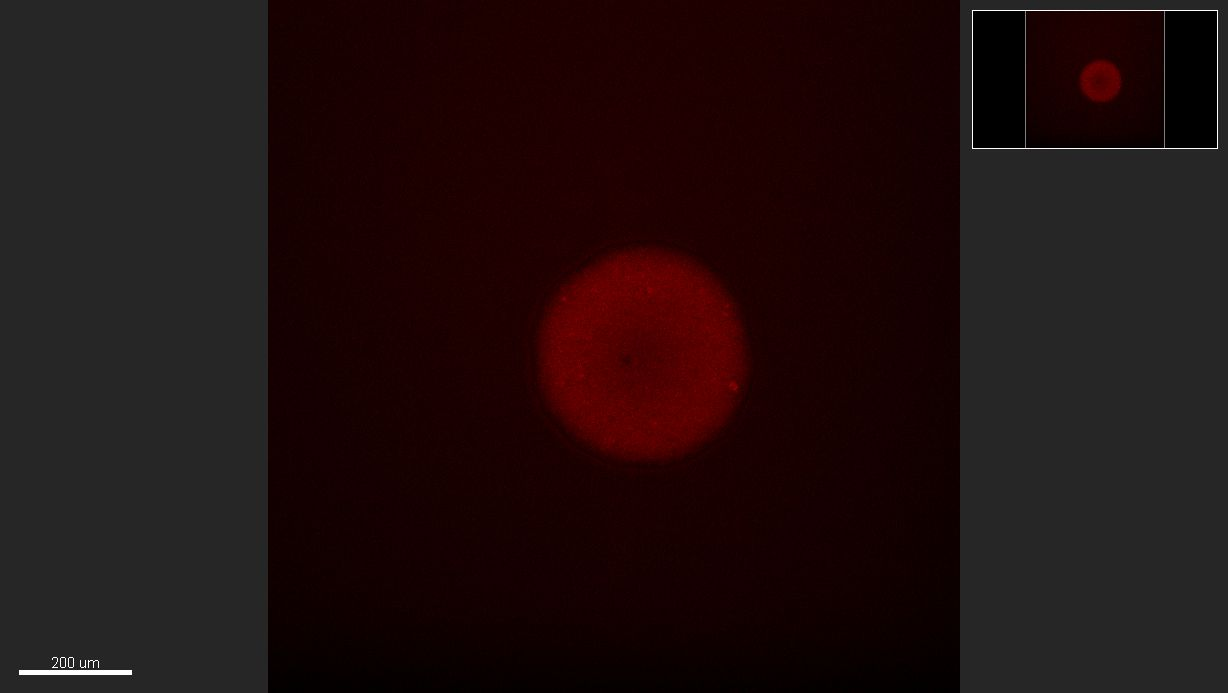
\includegraphics[width=0.25\linewidth]{CRASH/WT-rfp.jpg} &
        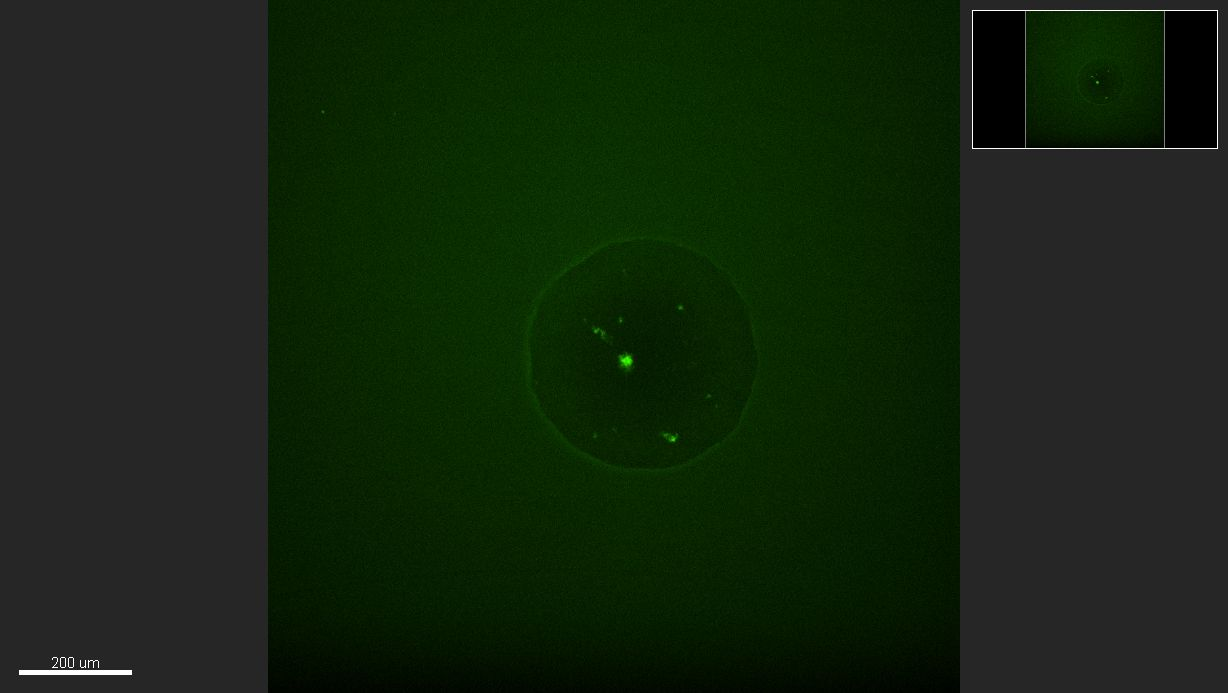
\includegraphics[width=0.25\linewidth]{CRASH/WT-gfp.jpg} &
        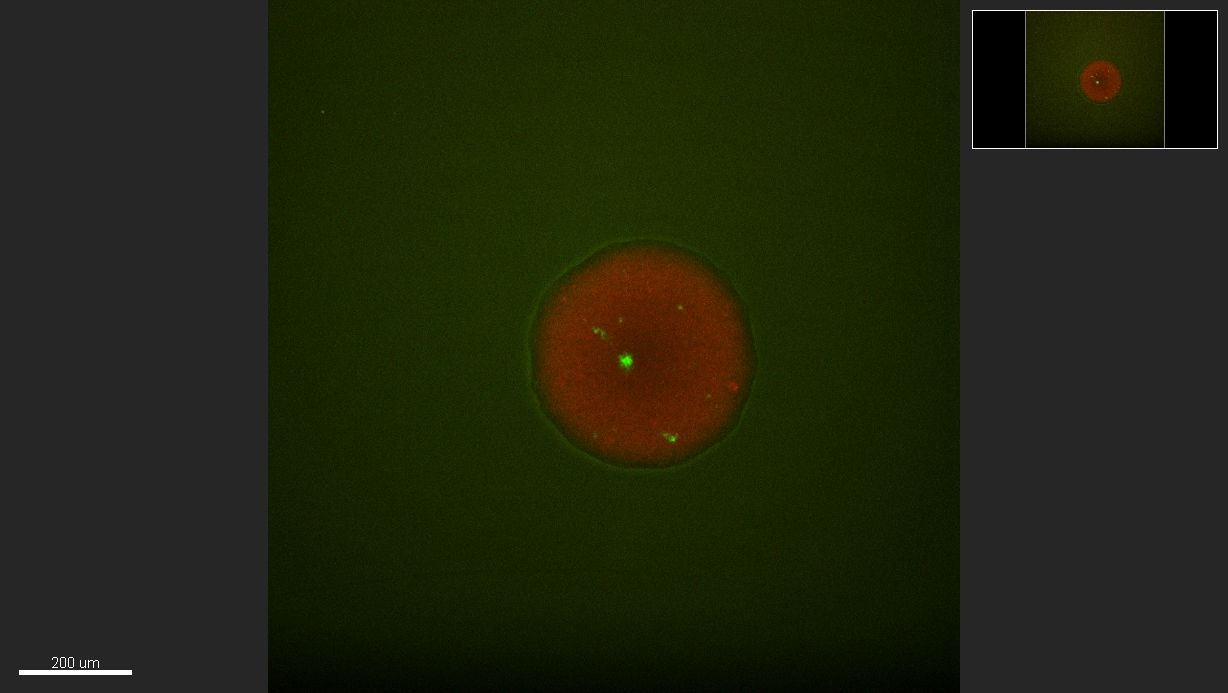
\includegraphics[width=0.25\linewidth]{CRASH/WT-merge.jpg} \\
        \hline

        \textbf{\textit{sir2}$\Delta$} &
        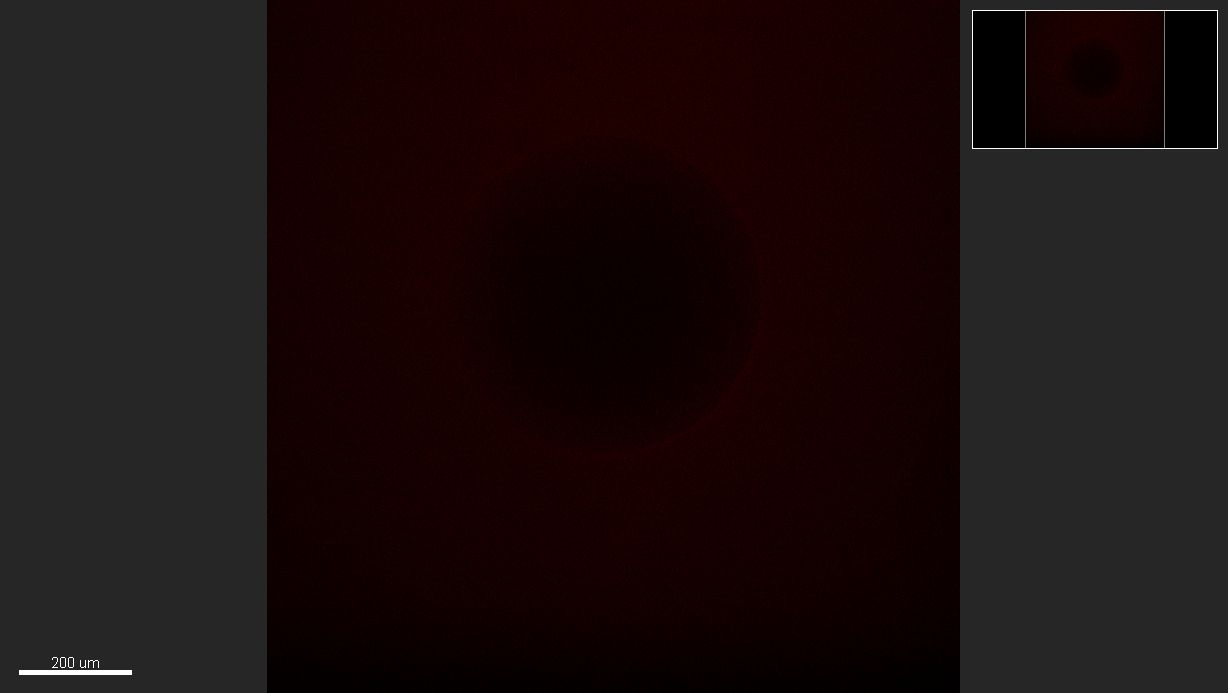
\includegraphics[width=0.25\linewidth]{CRASH/sir2delta-rfp.jpg} &
        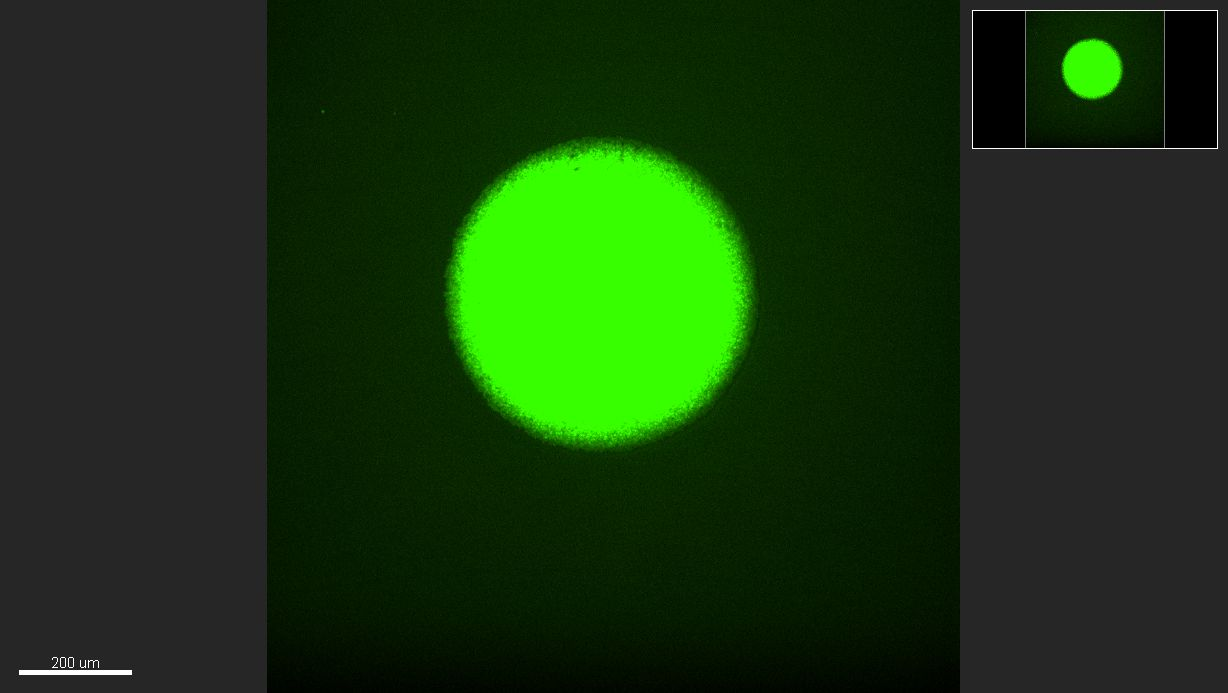
\includegraphics[width=0.25\linewidth]{CRASH/sir2delta-gfp.jpg} &
        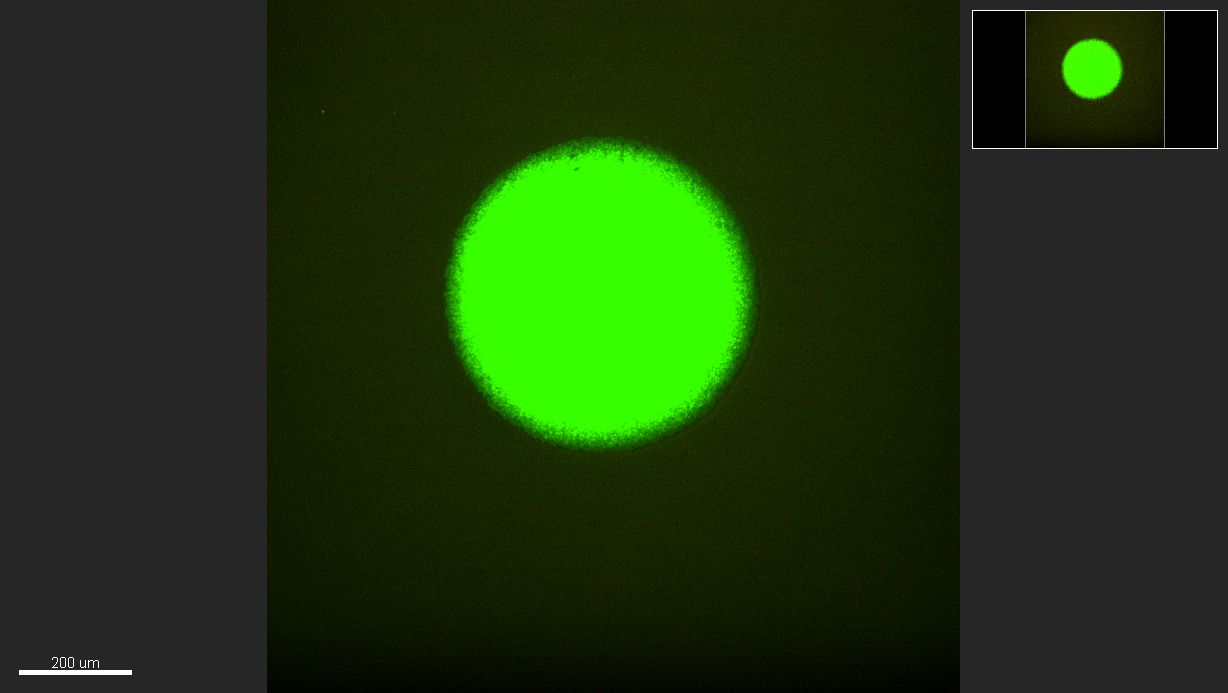
\includegraphics[width=0.25\linewidth]{CRASH/sir2delta-merge.jpg} \\
        \hline

        \textbf{$\Delta \alpha$ \textit{1-3}} &
        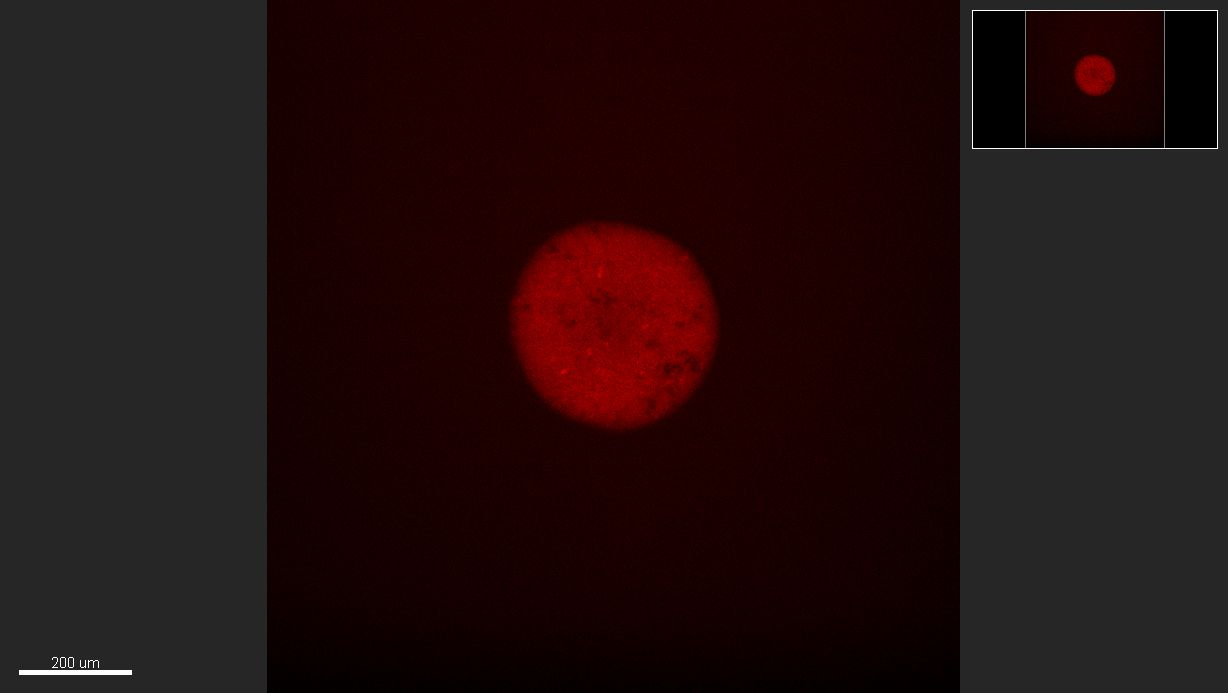
\includegraphics[width=0.25\linewidth]{CRASH/a13-rfp.jpg} &
        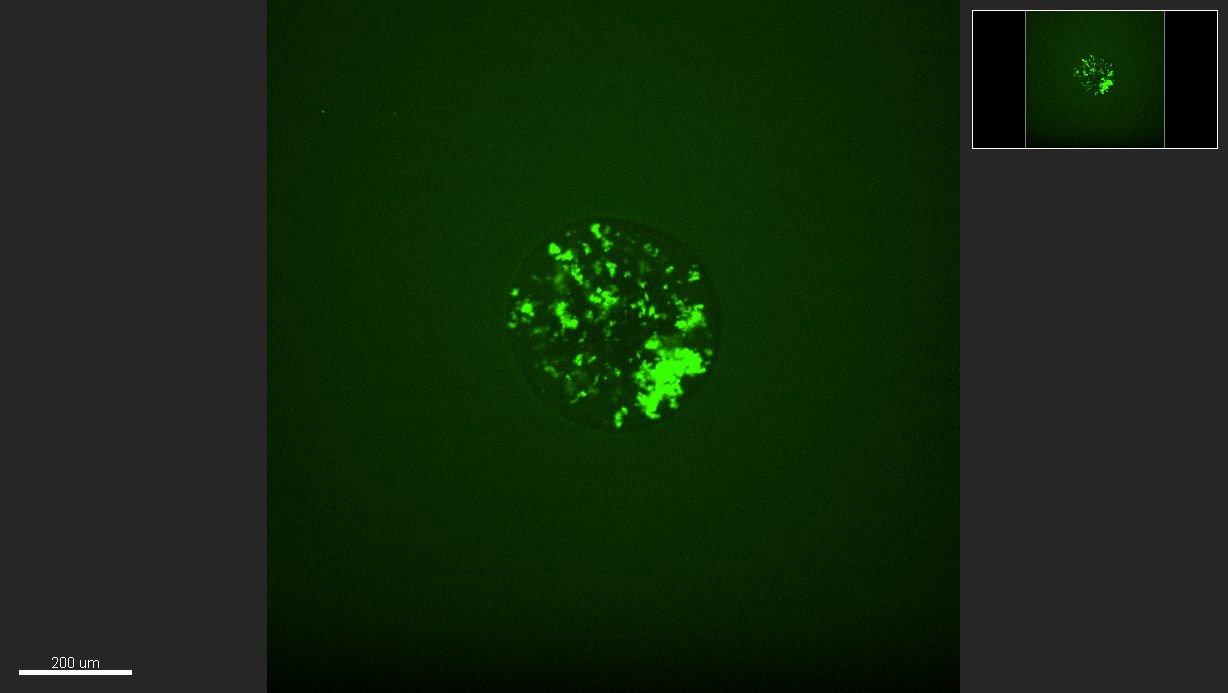
\includegraphics[width=0.25\linewidth]{CRASH/a13-gfp.jpg} &
        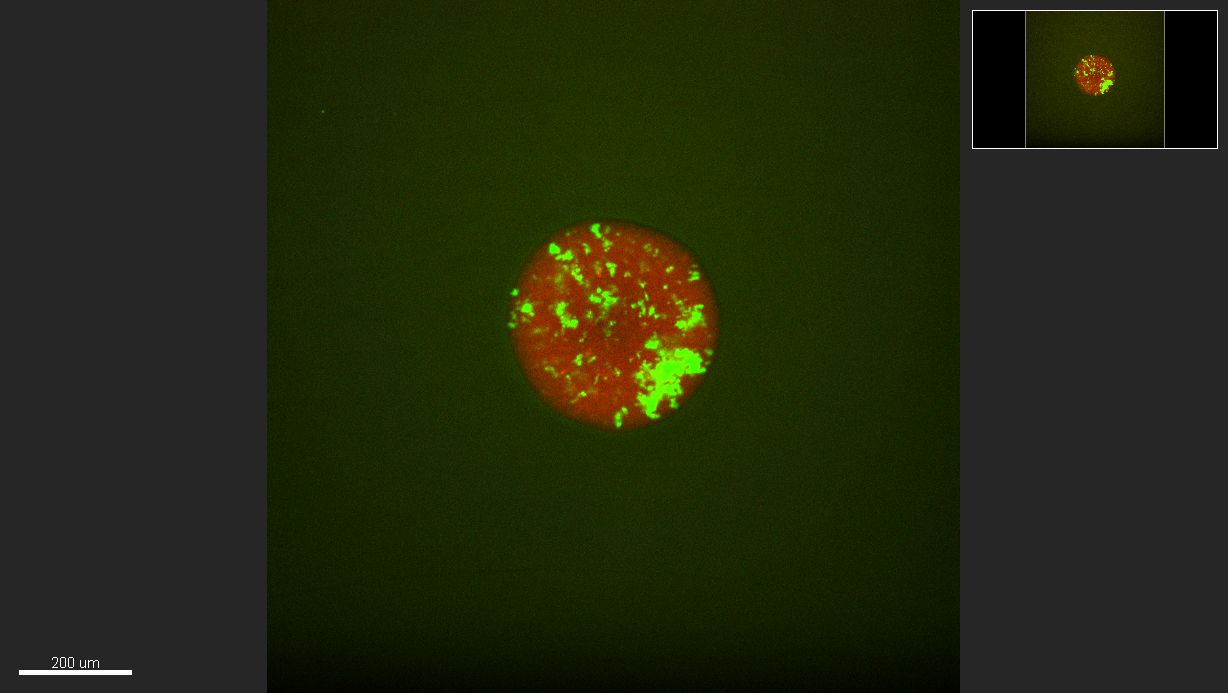
\includegraphics[width=0.25\linewidth]{CRASH/a13-merge.jpg} \\
        \hline

        \textbf{\textit{3A}} &
        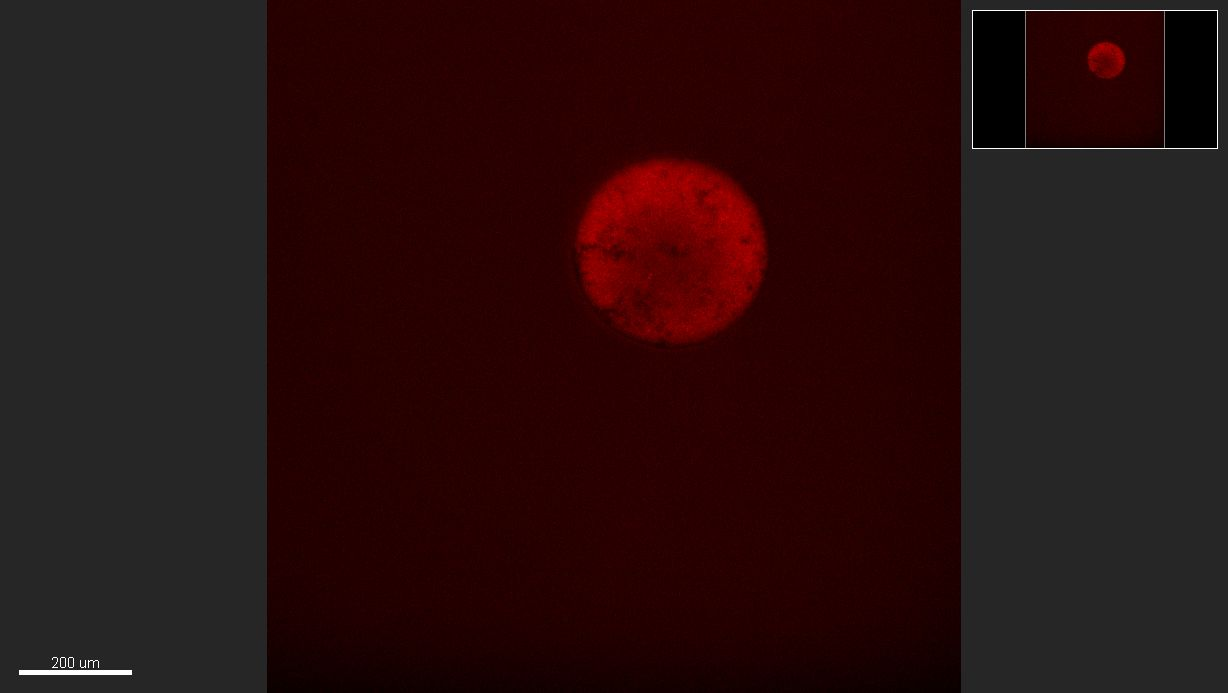
\includegraphics[width=0.25\linewidth]{CRASH/3A-rfp.jpg} &
        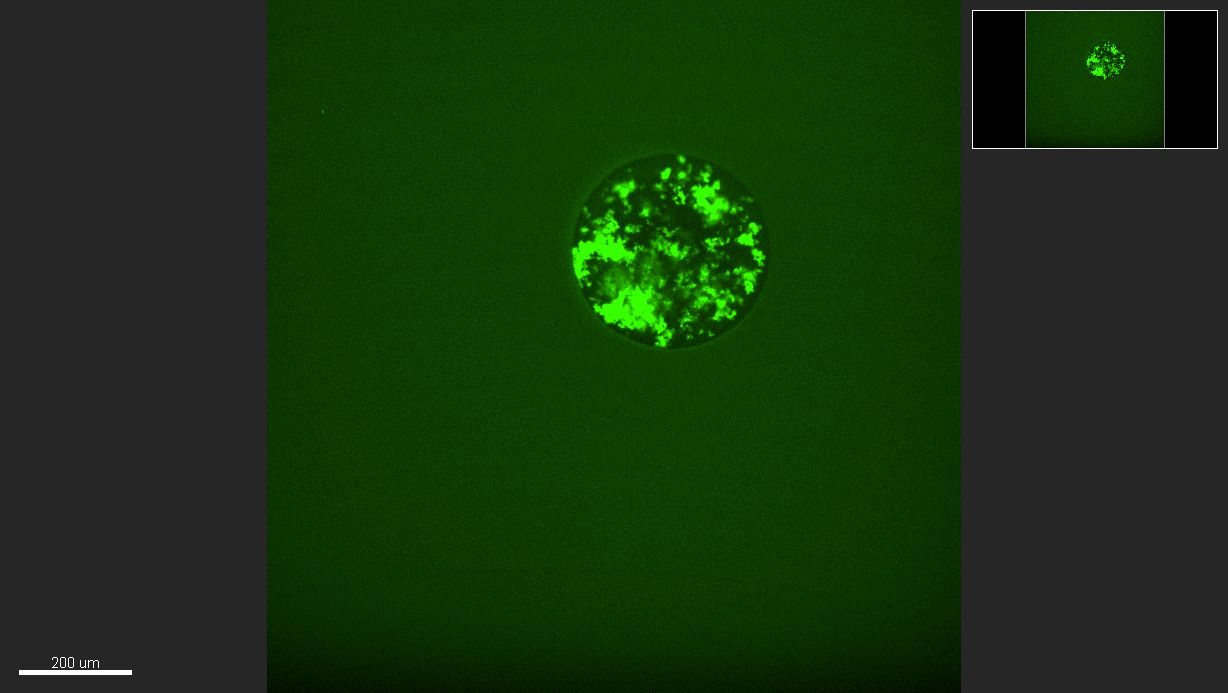
\includegraphics[width=0.25\linewidth]{CRASH/3A-gfp.jpg} &
        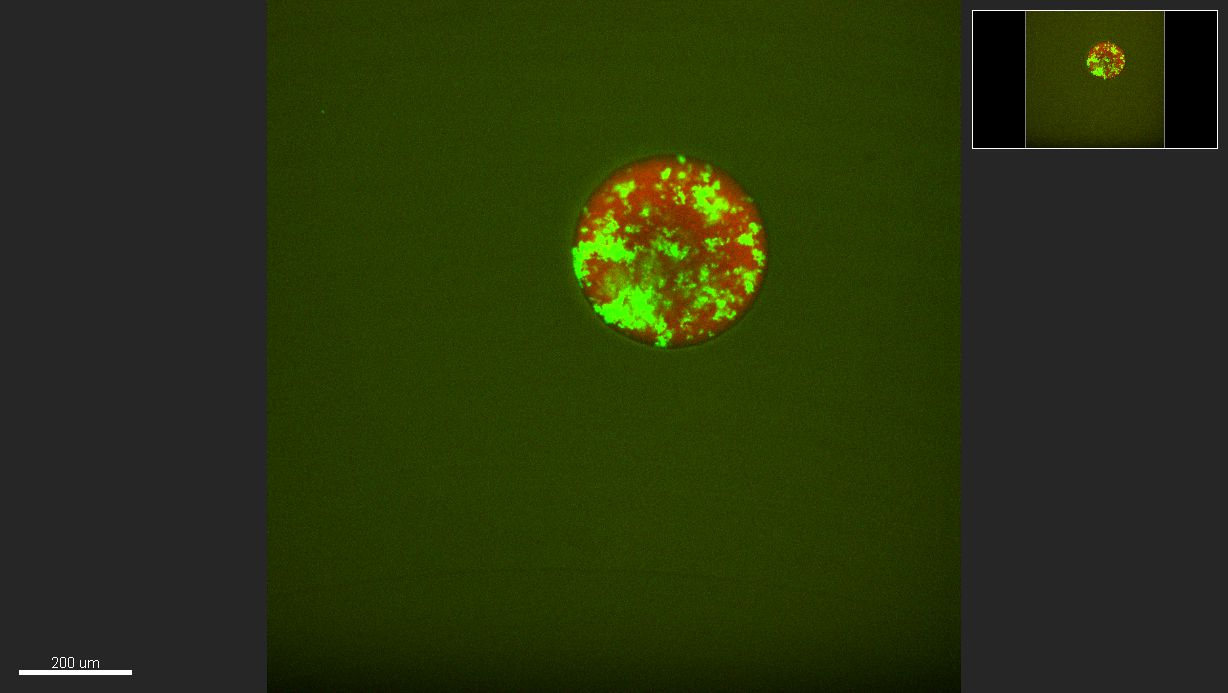
\includegraphics[width=0.25\linewidth]{CRASH/3A-merge.jpg} \\
        \hline

        \textbf{$\Delta \alpha$\textit{1-3 3A}} & 
        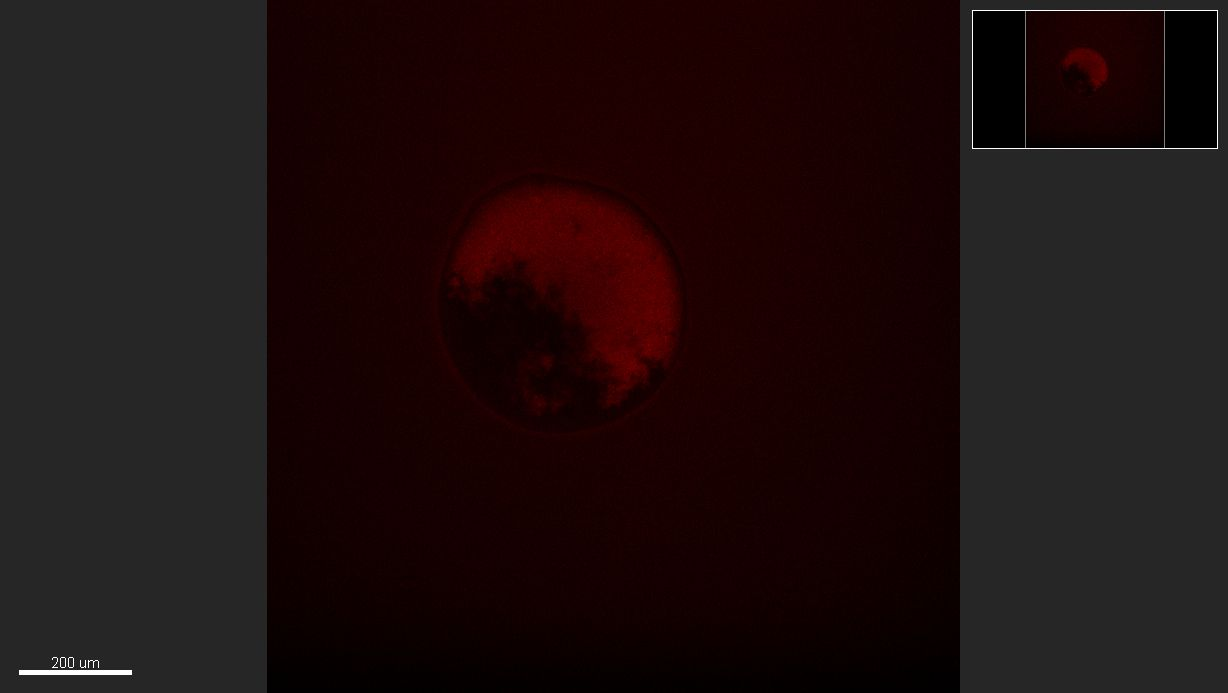
\includegraphics[width=0.25\linewidth]{CRASH/a13_3A-rfp.jpg} &
        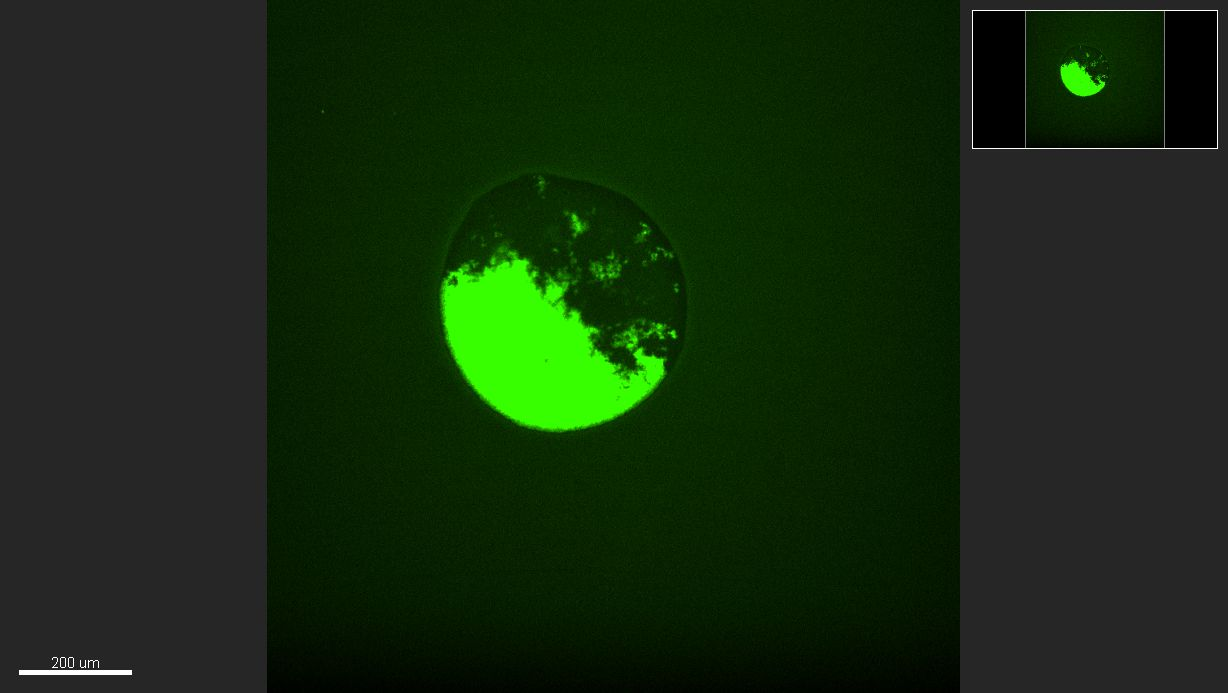
\includegraphics[width=0.25\linewidth]{CRASH/a13_3A-gfp.jpg} &
        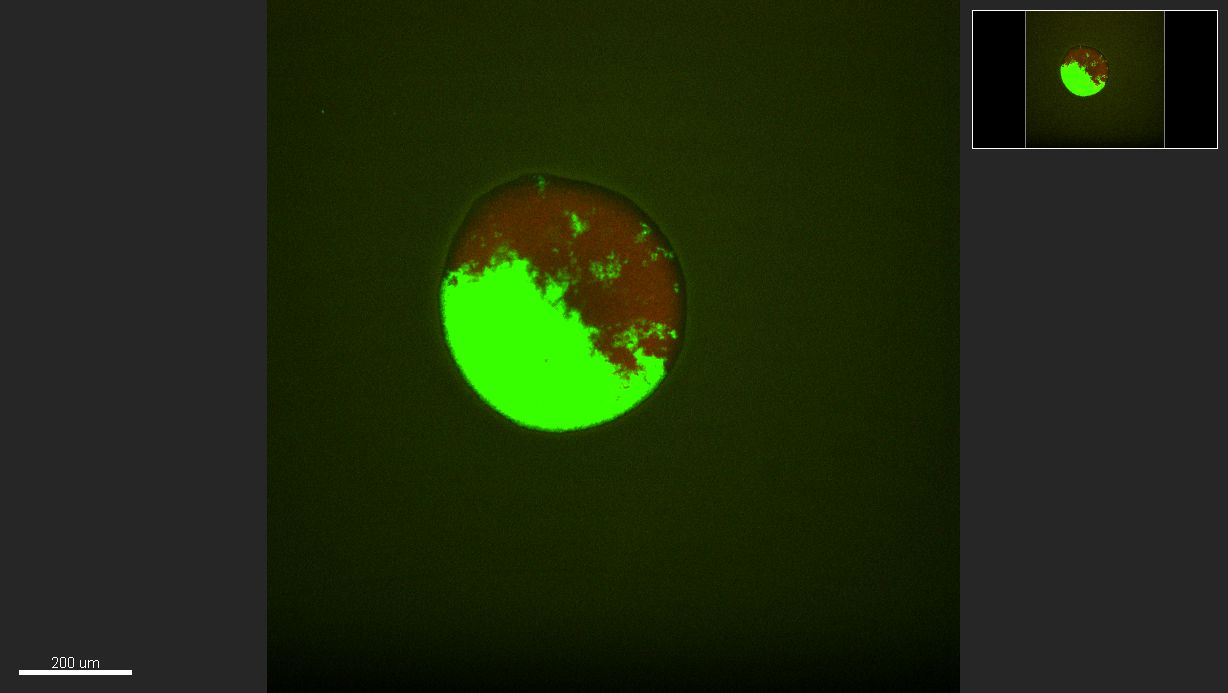
\includegraphics[width=0.25\linewidth]{CRASH/a13_3A-merge.jpg} \\
        \hline
    \end{tabular}
\end{table}

\subsection{流式细胞术定量分析}

采用的流式细胞仪定量分析CRASH体系菌株的荧光强度，结果如下：

\begin{table}[H]
    \centering
    \begin{tabular}{|c|c|c|c|c|c|}
        \hline
         & \textbf{wt} & \textbf{\textit{sir2A}} & \textbf{$\Delta \alpha$\textit{1-3}} & \textbf{\textit{3A}} & \textbf{$\Delta\alpha$\textit{1-3 3A}} \\
        \hline
        \textbf{RFP} & 98.3\% & 2.1\% & 83.8\% & 98.0\% & 97.2\%  \\
        \hline
        \textbf{GFP} & 0.2\% & 82.1\% & 13.8\% & 1.5\% & 1.5\% \\
        \hline
        \textbf{total} & 98.5\% & 84.2\% & 97.6\% & 99.5\% & 98.7\% \\
        \hline
    \end{tabular}
\end{table}

从定量结果来看，\textit{mcm2-3A}和\textit{mcm2-3A mrc1}突变表型依然以RFP$^+$为主，虽然确实造成了一部分酵母细胞异染色质沉默丢失，但是在数据上并不显著，同时双突变体并没有明显提升沉默缺陷的比例，两者相互协调增强效应并不明显，需要进一步研究确认。

\subsection{BiFC蛋白互作情况}
使用BiFC技术研究Mrc1蛋白中MLD $\alpha$1-3 区域与组蛋白互作情况，在普通明场和GFP通道下观察诱导前后突变型（$\Delta \alpha$\textit{1-3}）与野生型（wt）菌株，结果如下：

\begin{table}[htbp]
    \centering
    \begin{tabular}{|c|c|c|c|c|}
        \hline
        \multirow{3}{*}{} & \multicolumn{2}{c|}{\textbf{诱导前}} & \multicolumn{2}{c|}{\textbf{诱导后}} \\
        \cline{2-5}
         & \textbf{wt} & \textbf{\textit{$\Delta\alpha$1-3}} & \textbf{wt} & \textbf{\textit{$\Delta\alpha$1-3}} \\
        \hline
        \textbf{Bright} & 
        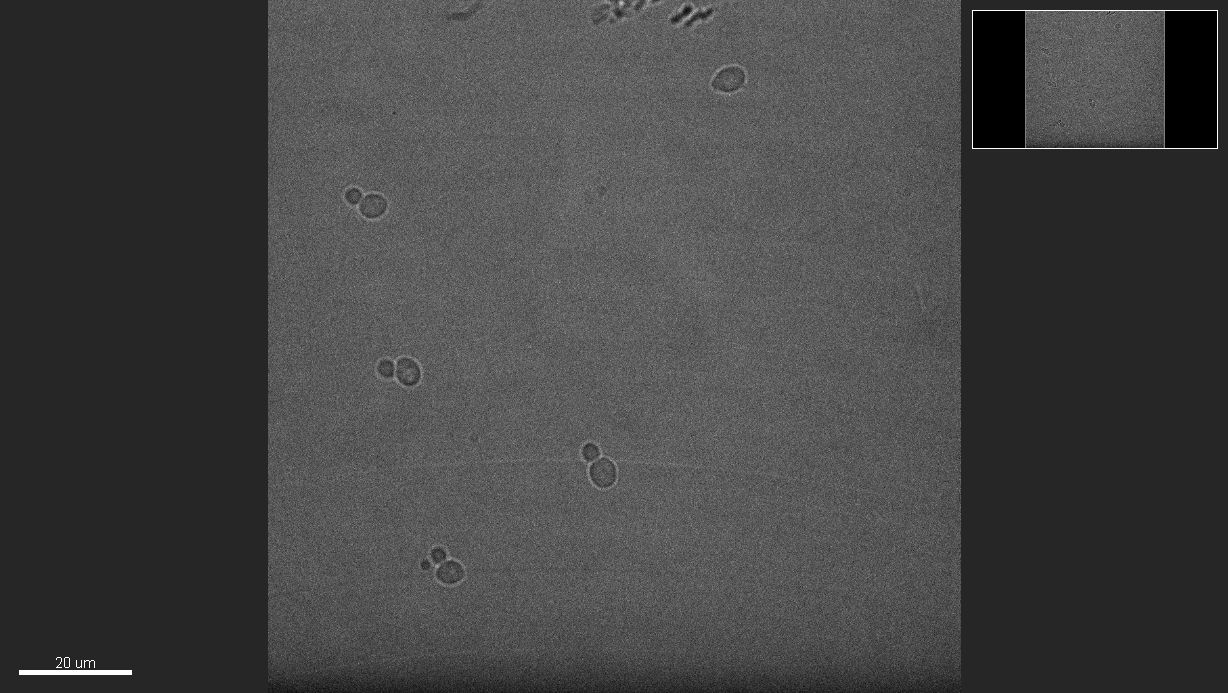
\includegraphics[width=0.18\linewidth]{BiFC/Comparison/wt-light.jpg} & 
        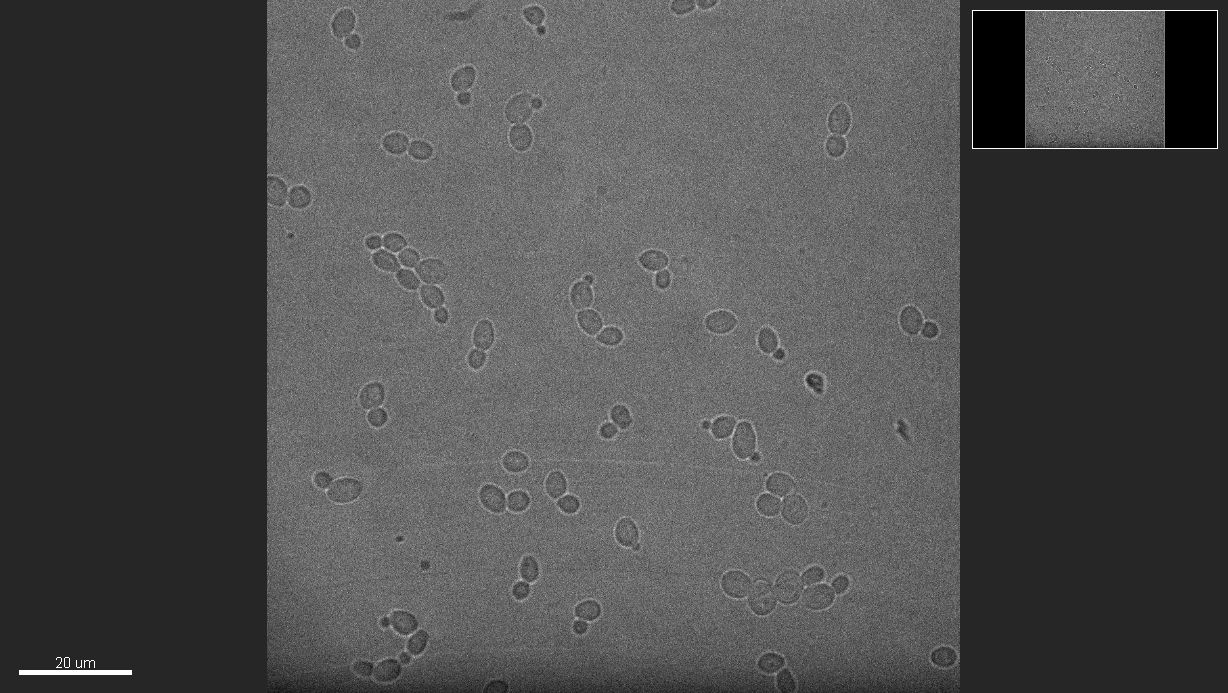
\includegraphics[width=0.18\linewidth]{BiFC/Comparison/da-light.jpg} & 
        
\includegraphics[width=0.18\linewidth]{BiFC/Experimental/wt-light.jpg} &
        
\includegraphics[width=0.18\linewidth]{BiFC/Experimental/da-light.jpg} \\
        \hline
        \textbf{GFP} & 
        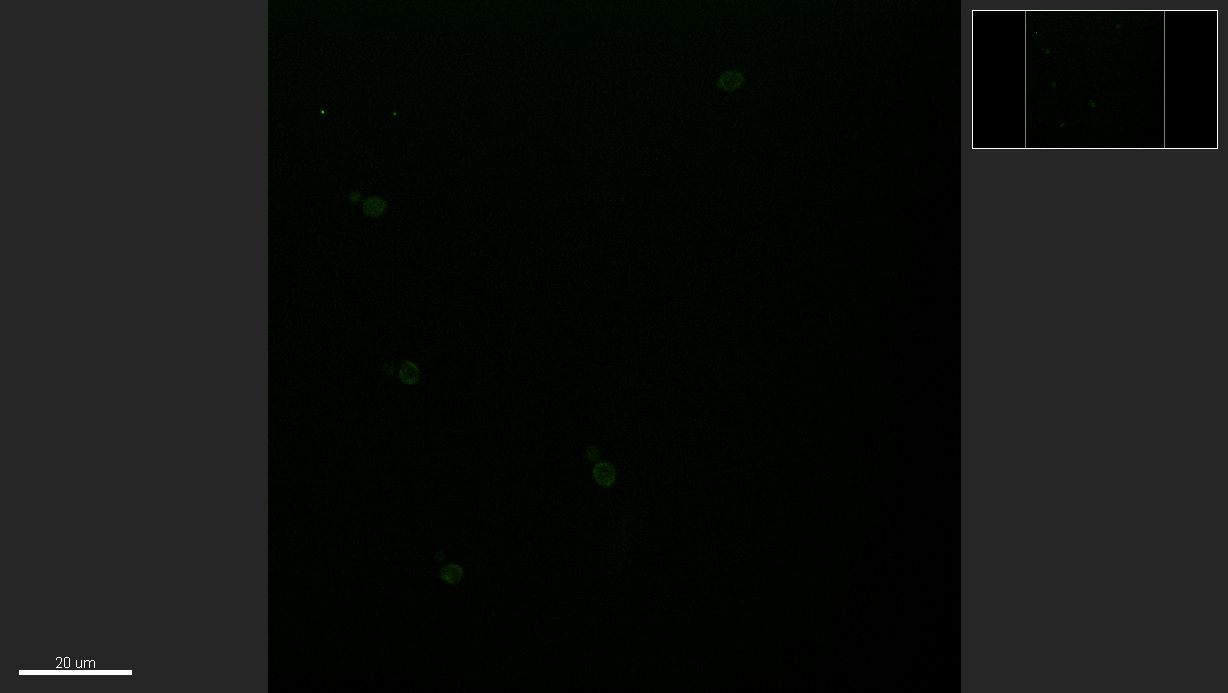
\includegraphics[width=0.18\linewidth]{BiFC/Comparison/wt-gfp.jpg} & 
        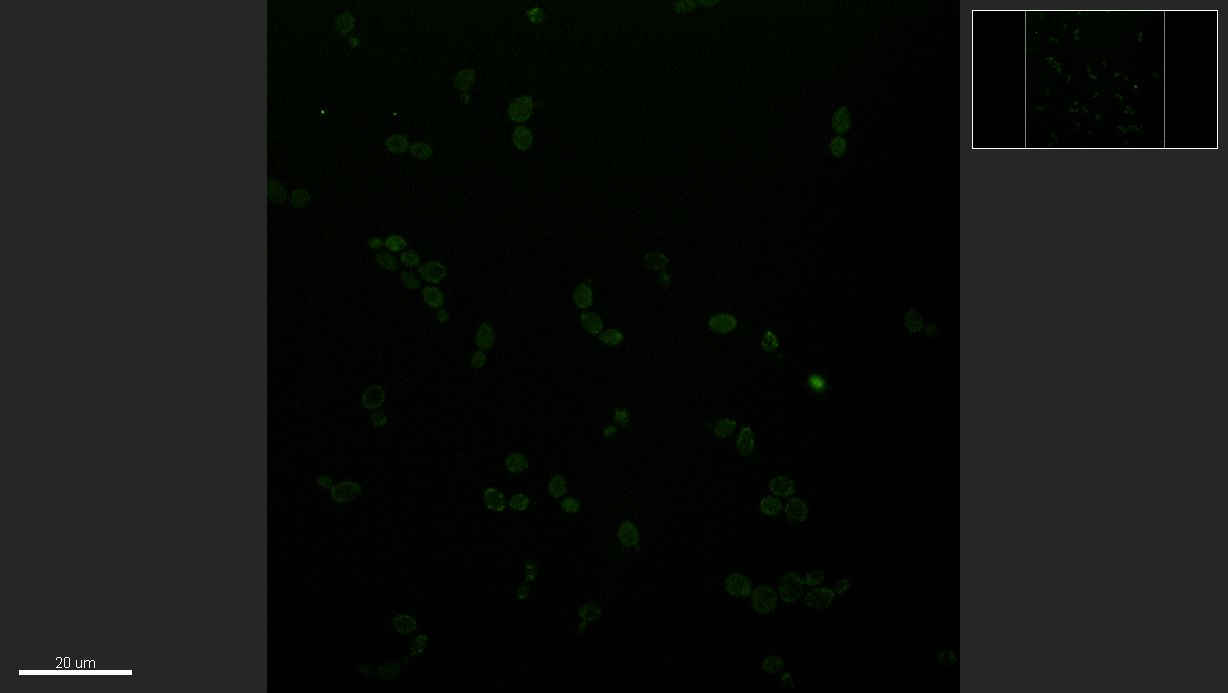
\includegraphics[width=0.18\linewidth]{BiFC/Comparison/da-gfp.jpg} & 
        
\includegraphics[width=0.18\linewidth]{BiFC/Experimental/wt-gfp.jpg} & 
        
\includegraphics[width=0.18\linewidth]{BiFC/Experimental/da-gfp.jpg} \\
        \hline
        \textbf{Merge} & 
        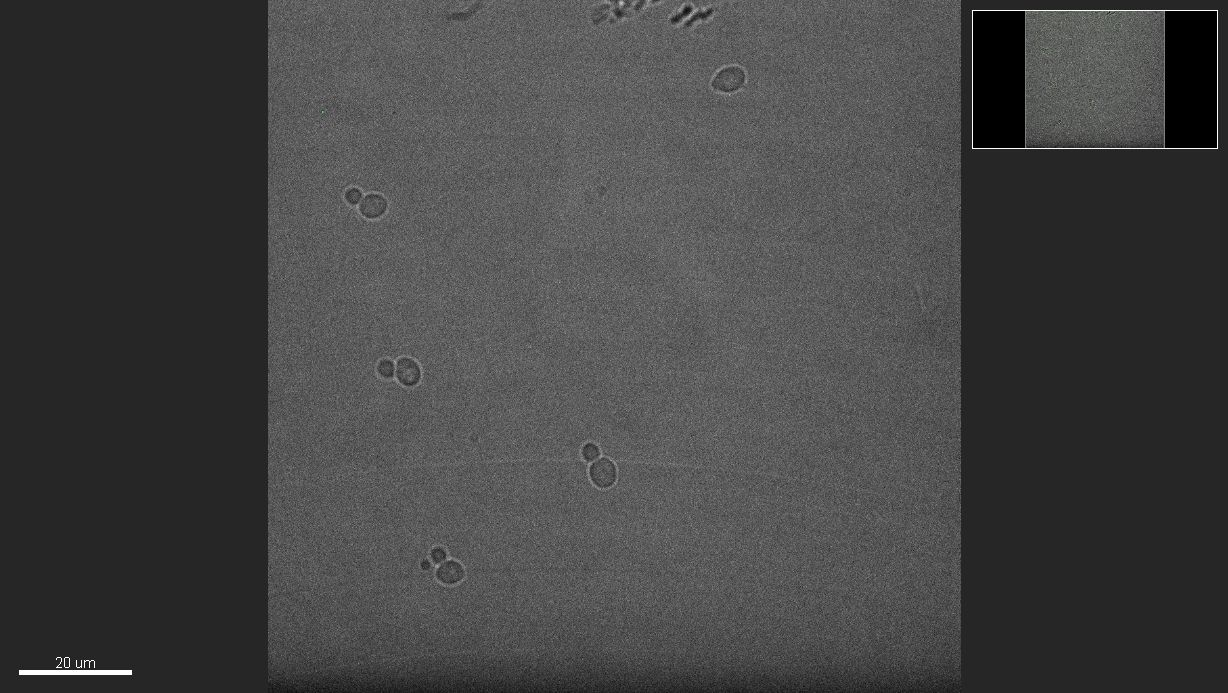
\includegraphics[width=0.18\linewidth]{BiFC/Comparison/wt-merge.jpg} & 
        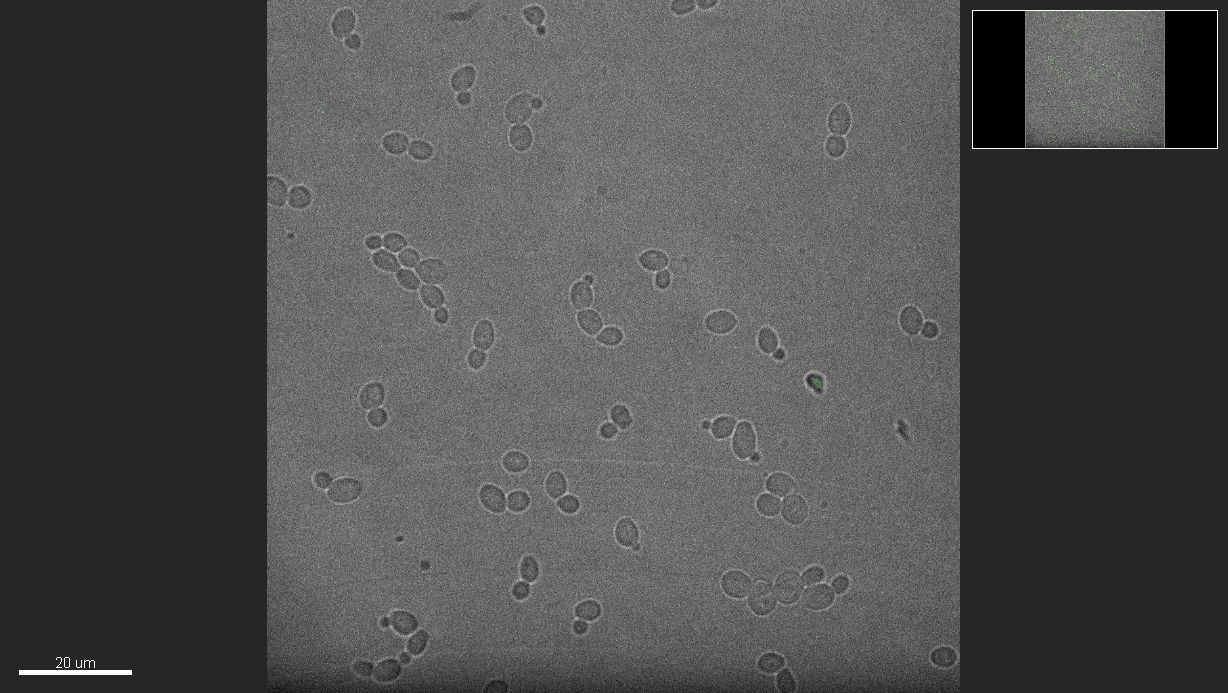
\includegraphics[width=0.18\linewidth]{BiFC/Comparison/da-merge.jpg} & 
        
\includegraphics[width=0.18\linewidth]{BiFC/Experimental/wt-merge.jpg} & 
        
\includegraphics[width=0.18\linewidth]{BiFC/Experimental/da-merge.jpg} \\
        \hline
    \end{tabular}
\end{table}

观察到诱导前后突变型与野生型菌株都未激发产生绿色荧光，说明MLD $\alpha$ 1-3区域未能与组蛋白产生有效互作。检查实验流程，发现在诱导质粒表达时选用了 \qty{30}{\celsius} 摇床培养，并非质粒最佳表达条件，导致酵母质粒未能正常表达，造成荧光信号缺失。

\subsection{结论}
通过CRASH体系荧光研究可以初步判断Mrc1在控制细胞表观信息稳定性中起到一定作用，但是具体组蛋白H3-H4作用机制还需要进一步研究。

\clearpage
\printbibliography[title={参考文献}]

\end{document}